\documentclass[../main.tex]{subfiles}
\graphicspath{{\subfix{../images/}}}
\begin{document}
\section*{Term 1 Week 9}
\begin{enumerate}
    \item 
    Change each log to base 2:\\
    \(\frac{1}{\frac{\log_2(x)}{\log_2(8)}}+\frac{1}{\frac{\log_2(\frac{1}{4}}{\log_2(x)}}=-\frac{5}{2}\)\\

    \(\frac{3}{\log_2(x)}+\frac{\log_2(x)}{-2}=-\frac{5}{2}\)\\

    \(\frac{3}{\log_2(x)}-\frac{\log_2(x)}{2}=-\frac{5}{2}\)\\

    Turn it into a quadratic:\\
    \(\frac{3}{\log_2(x)}-\frac{\log_2(x)}{2}=-\frac{5}{2}\)\\

    \(\frac{6}{\log_2(x)}-\log_2(x)=-5\)\\

    \(6-(\log_2(x))^2=-5\log_2(x)\)\\

    \((\log_2(x))^2-5\log_2(x)-6=0\)\\

    Solving:\\
    \(\log_2(x)=\frac{5\pm \sqrt{49}}{2}\)\\

    \(\log_2(x)=\frac{5\pm 7}{2}=6,-1\)\\

    \(\log_2(x)=6\\
    x=2^6=64\\
    \)\\
    \(
    \log_2(x)=-1\\
    x=2^{-1}=\frac{1}{2}
    \)
    

    \item
    Firstly, remember that \(V=\pi r^2 h\) and the radius is constant, therefore \(\frac{dV}{dh}=\pi r^2\)\\
    \(\frac{dV}{dt}=-k\sqrt{h}\)\\
    By the Chain Rule:
    \(\frac{dV}{dt}=\frac{dV}{dh}\times \frac{dh}{dt}\)\\

    Therefore, \(-k\sqrt{h}=\pi r^2 \times \frac{dh}{dt}\)\\
    \(\frac{dh}{dt}=-\frac{k\sqrt{h}}{\pi r^2}\)\\

    Separate variables and integrate:\\
    \(\frac{1}{\sqrt{h}}dh=-\frac{k}{\pi r^2} dt\)\\
    \(\int \frac{1}{\sqrt{h}}dh=\int -\frac{k}{\pi r^2} dt\)\\
    \(2\sqrt{h}=-\frac{k}{\pi r^2}t+c\)\\

    At \(t=0, h=1\):\\
    \(2\sqrt{1}=-\frac{k}{\pi r^2}(0)+c\), therefore \(c=2\)\\
    
    \(2\sqrt{h}=-\frac{k}{\pi r^2}t+2\)\\

    At \(t=1, h=\frac{1}{2}\):\\
    \(2\sqrt{\frac{1}{2}}=-\frac{k}{\pi r^2}+2\)\\

    \(\frac{k}{\pi r^2}=2-2\sqrt{\frac{1}{2}}\)\\

    \(k=\pi r^2(2-2\sqrt{\frac{1}{2}})\)\\

    Substituting back into the model:\\
     \(2\sqrt{h}=-\frac{\pi r^2(2-2\sqrt{\frac{1}{2}})}{\pi r^2}t+2\)\\

    \(2\sqrt{h}=-(2-2\sqrt{\frac{1}{2}})t+2\)\\

     \(2\sqrt{h}=(2\sqrt{\frac{1}{2}}-2)t+2\)\\

     \(\sqrt{h}=(\sqrt{\frac{1}{2}}-1)t+1\)\\

     Solve for \(t\) when \(h=0\):\\
     \((\sqrt{\frac{1}{2}}-1)t+1=0\)\\

     \((\sqrt{\frac{1}{2}}-1)t=-1\)\\

    \(t=\frac{1}{\sqrt{\frac{1}{2}}}=\frac{1}{\frac{\sqrt{2}-1}{\sqrt{2}}}=\frac{\sqrt{2}}{\sqrt{2}-1}=\sqrt{2}+2=3.414\)\\    

    \item 
    Differentiate:\\
    \(y'=-\frac{x}{\sqrt{2\pi}}e^{-\frac{x^2}{2}}\)\\

    Differentiate a second time using the product rule:\\
    \(y''=-\frac{1}{\sqrt{2\pi}}e^{-\frac{x^2}{2}}+\frac{x^2}{\sqrt{2\pi}}e^{-\frac{x^2}{2}}\)\\

    To find the steepest point, make it equal to zero and solve for x:\\
    \(\frac{e^{-\frac{x^2}{2}}}{\sqrt{2\pi}}(x^2-1)=0\)\\

    Since \(e^{-\frac{x^2}{2}}\) can never equal zero:\\
    \(x^2-1=0\)\\
    \(x=\pm 1\)\\

    Substituting back into the original equation to get the y-coordinates:\\
    \(y=\frac{1}{\sqrt{2\pi}}e^{-\frac{1}{2}}=\frac{1}{\sqrt{2\pi}}\times \frac{1}{\sqrt{e}}=\frac{1}{\sqrt{2\pi e}}\)
    \begin{figure}[H]
        \centering
        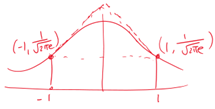
\includegraphics[width=0.25\linewidth]{images/t1w9q3_a.png}
    \end{figure}
    Get the gradients of each line:\\
    \(x=1: y'=-\frac{1}{\sqrt{2\pi}}e^{-\frac{1^2}{2}}=-\frac{1}{\sqrt{2\pi e}}\)\\
    \(x=-1: y'=\frac{1}{\sqrt{2\pi}}e^{-\frac{(-1)^2}{2}}=\frac{1}{\sqrt{2\pi e}}\)\\

    Get the y-intercept (and the +c of each equation):\\
    \(\frac{1}{\sqrt{2\pi e}}=-\frac{1}{\sqrt{2\pi e}}\times 1+c\)\\
    \(c=\frac{2}{\sqrt{2\pi e}}\)\\
    \(y=-\frac{x}{\sqrt{2\pi e}}+\frac{2}{\sqrt{2\pi e}}\)\\
    Get the x-intercept by y=0:\\
    \(0=-\frac{x}{\sqrt{2\pi e}}+\frac{2}{\sqrt{2\pi e}}\)\\
    \(\frac{x}{\sqrt{2\pi e}}=\frac{2}{\sqrt{2\pi e}}\)\\
    \(x=2\)\\

    \(\frac{1}{\sqrt{2\pi e}}=\frac{1}{\sqrt{2\pi e}}\times -1+c\)\\
    \(c=\frac{2}{\sqrt{2\pi e}}\)\\
    \(y=\frac{x}{\sqrt{2\pi e}}+\frac{2}{\sqrt{2\pi e}}\)\\
    Get the x-intercept by y=0:\\
    \(0=\frac{x}{\sqrt{2\pi e}}+\frac{2}{\sqrt{2\pi e}}\)\\
    \(\frac{x}{\sqrt{2\pi e}}=-\frac{2}{\sqrt{2\pi e}}\)\\
    \(x=-2\)
    \begin{figure}[H]
        \centering
        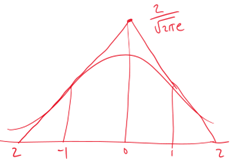
\includegraphics[width=0.25\linewidth]{images/t1w9q3_a2.png}
    \end{figure}
    Base of triangle is 4, height is \(\frac{2}{\sqrt{2\pi e}}\)\\
    Area = \(\frac{1}{2}\times 4 \times \frac{2}{\sqrt{2\pi e}}= \frac{4}{\sqrt{2\pi e}}=\frac{\sqrt{16}}{\sqrt{2\pi e}}=\sqrt{\frac{8}{\pi e}}\)
    
\end{enumerate}

\end{document}